\begin{section}{Resultados}

	Para analizar las diferencias y/o similitudes en la aplicación práctica de los tres algoritmos implementados se generaron gráficos que pasan a detallarse a continuación. 
		
	El primero de ellos consiste en gráficar el error relativo en función de la cantidad de iteraciones para cada uno de los algoritmos. Se utilizó precisión fija de 51 bits ya que por precondición la cantidad de dígitos de la mantisa debe ser menor a 52, es decir, con 51 dígitos minimizamos el error. Conseguimos la precisión deseada mediante truncamiento.
	El eje del gráfico que corresponde al $error\;relativo$ está en escala logarítmica para poder apreciar mejor los valores correspondientes dado que estos decrecen exponencialmente.

	\begin{figure}[H]
	  \centering
		\includegraphics[width=10cm,angle=-90]{graficos/comparacion_1a42it_51p.eps}
	  \caption{Comparación del error relativo de las tres series variando de 1 a 42 la cantidad de términos calculados con precisión de 51 bits en la mantisa.}
	  \label{fig:51p}
	\end{figure}
	
	\VSP

	Para un posterior análisis sobre la información aquí suministrada, se agrega a continuación, un gráfico, detalle del anterior, se mostrará el error relativo entre la iteración 3 y 12 para el algoritmo de $Machin$ y el de $Ramanujan$ con los mismos parámetros (51 digitos de precisión).
	
	\begin{figure}[H]
	  \centering
		\includegraphics[width=10cm,angle=-90]{graficos/comparacion_machin-ram.eps}
	  \caption{Comparación del error relativo la serie de Machin y de Ramanujan variando de 3 y 12 la cantidad de términos calculados con precisión de 51 bits en la mantisa.}
	  \label{fig:greg-ram}
	\end{figure}
	
	\VSP
	
	Se realizaron además, experimentaciones sobre el error relativo en función de la cantidad de bits de precisión (variando este parámetro de 1 a 51). A continuación se detallan los resultados de estos experimientos.
	
	Se corrieron las pruebas hasta 42 iteraciones debido a que la serie de $Ramanujan$ es informativa hasta esa iteración (a partir de 43 iteraciones devuelve $nan$), es decir, el error relativo presentado corresponde al error cometido al calcular 42 términos de la serie.
	
	El gráfico se presenta bajo una escala logarítmica en $y$.
	
	\begin{figure}[H]
	  \centering
		\includegraphics[width=10cm,angle=-90]{graficos/comparacion_42it_1a51p.eps}
	  \caption{Comparación del error relativo de las tres series en el término 42 variando de 1 y 51 la cantidad de bits en la mantisa.}
	  \label{fig:42it}
	\end{figure}
	
	\VSP
	
	Consideramos que es pertinente mostrar un nuevo gráfico fijando la cantidad de iteraciones en un valor menor para verificar si existe alguna diferencia o no. Elegimos arbitrariamente correr las pruebas con 5 iteraciones.
	
	\begin{figure}[H]
	  \centering
		\includegraphics[width=10cm,angle=-90]{graficos/comparacion_5it_1a51p.eps}
	  \caption{Comparación del error relativo de las tres series en el término 5 variando de 1 y 51 la cantidad de bits en la mantisa.}
	  \label{fig:5it}
	\end{figure}
	
	\VSP
	
	NOTA: 
	
	Para hacer más simple el análisis de los gráficos, cada par de valores correspondientes a puntos consecutivos del eje $x$, se los unió mediante una recta, funcionalidad utilizada de GNUPLOT.
	
	No se utilizaron polinomios interpoladores para aproximar por la curva o recta que pase por todos los puntos correspondiente a una misma fuente de datos, estas conclusiones fueron sacadas utilizando experimentación empírica, suponiendo que el comportamiento cuando los valores del eje $x$ tienden a infinito se corresponden a los de los valores graficados.\\

	El último gráfico corresponde al error relativo en función de la cantidad de dígitos, pero evaluando las cotas obtenidas en el análisis teórico con el error relativo de implementación.
	
	La información obtenida en este gráfico, nos ayudará a poder discernir cuál es la relación que existe entre estos dos mundos.
	
	\begin{figure}[H]
	  \centering
		\includegraphics[width=10cm,angle=-90]{graficos/cotas.eps}
	  \caption{Comparación del error relativo de las tres series y los errores teóricos en función de la cantidad de bits de mantisa.}
	  \label{fig:cotas}
	\end{figure}
\end{section}
